% Basic LaTeX template for NE 204 lab report
\documentclass[11pt]{article}

%==============================================================================
%%% Everything between the "="'s is the preamble.
%%% Define packages and meta data here

% Common packages
\usepackage{amsmath}    % Expanded math
\usepackage{amssymb}    % Expanded math symbols
\usepackage{graphicx}   % For images
%\usepackage[version=3]{mhchem} % For nuclide formatting

% All images/figures will be stored in the images folder.
% Specify that here so pdflatex knows where to look for images.
\graphicspath{{./images/}}

% Metadata
\title{Two-point Calibration of a Coaxial HPGe Detector}
\author{Jake Hecla}
\date{January 31, 2018}
%==============================================================================

\begin{document}

% Compile metadata from preamble into a nicely-rendered title section
\maketitle

% The *'s next so section/subsection definitions suppresses numbering
\section*{Introduction}
\label{sec:intro}
High purity germanium (HPGe) detectors offer a means of high energy resolution gamma
ray counting and are considered the gold standard for lab-scale gamma
spectroscopy(citation). These detectors require constant crogenic cooling when in use to
diminish thermal promotion of charge carriers to the conduction band{citation}. As a
result of thermal cycling and drift in readout electronics, these detectors must
be regularly energy calibrated. This is typically carried out using a number of
check sources which span the range of gamma ray energies one is likely to encounter
in everyday life (~.05-2MeV). \par
While calibration can theoretically be carried out using a minimum of two distinct
photopeaks, standard operating procedures in most cases call for at least three
of such peaks spaced widely across the useful energy range. This approach minimizes
error and provides information on the linearity of the detector's energy response. \par
In this lab, we process spectra from three distinct sources (cesium-137, americium-241
and barium-133) and use the channel numbers associated with the Cs and Am photopeaks
to develop a two-point energy calibration model. We then apply this calibration to the
barium-133 spectrum, which shows small errors (order of 1keV) in energy calibration in the
~300-500keV range. 


\section*{Methods}
\label{sec:meth}
Spectra resulting from measurements of Co-60, Am-241, Cs-137,and Ba-133 check
sources were provided to students via a publicly-accessible dropbox folder. Via
a python script, this data was downloaded and placed in NumPy arrays for
analysis. Peaks in the spectra corresponding to photopeaks of known energy were
then picked out manually and fitted using a gaussian distribution using SciPy's
curvefit tool. The estimates produced by curvefit for /mu (in units of channel number) for the
661.7keV and 59.5keV lines from the Cs and Am sources were then
used to develop a linear calibration of the form \[E_x = a*x + b\] (in which x denotes
the channel index).This calibration was then applied to the dataset gathered from
a Ba-133 check source in order to determine the accuracy of the fit.


\section*{Results and Discussion}
\label{sec:res}
The application of the calibration derived from the 59.5keV Am line and the
661.7keV Cs line to the Ba-133 dataset showed close agreement with data
on the energy of the gamma rays emitted in its decay.
The largest deviation
was observed for the 356keV line, which is off by approximately 1keV. This is
a surprisingly good result considering that this is a two-point calibration in
a large-volume detector with known poor performance at low energies due to
incomplete charge collection. Further research using a multiline calibration
and more low-energy sources should provide more information about the reliability
of this calibration at the extreme edges of this detector's useful energy range.

\begin{figure}[h]
  \centering
  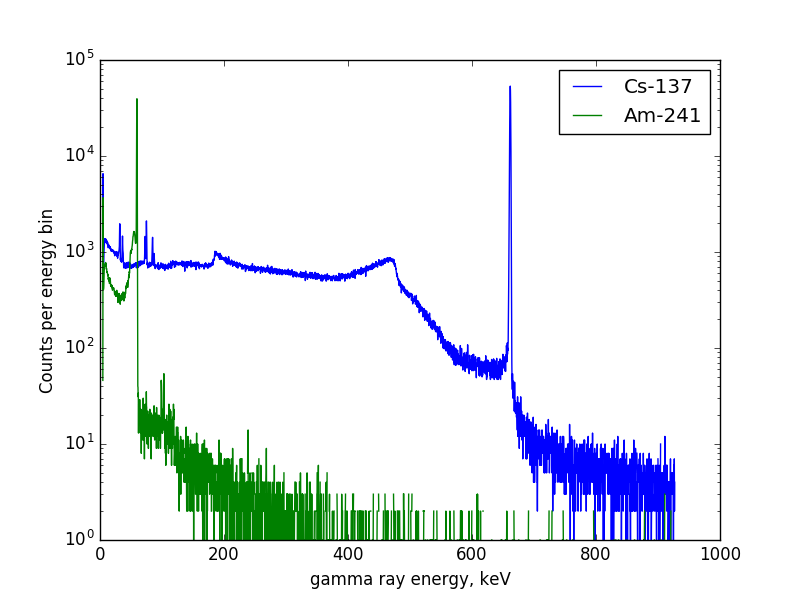
\includegraphics[width=0.7\textwidth]{cs_ba}
  \caption{This histogram is the result of applying the two-point calibration
  derived from the 59.5keV and 661.7keV photopeaks to the Cs and Am data. }
\label{fig:cesiumamericium}
\end{figure}

\begin{figure}[h]
  \centering
  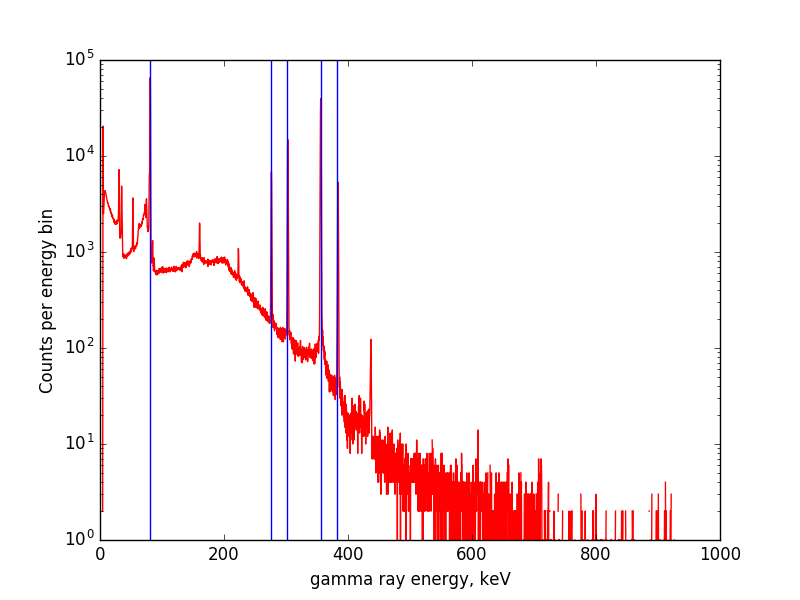
\includegraphics[width=0.7\textwidth]{Ba_data_check}
  \caption{Applying the two-point calibration to the Ba-133 data as shown above
  gives excellent agreement with data from NNDC on the energies of the
  gamma rays emitted in its decay (indicated by vertical lines). }
\label{fig:bariumcal}
\end{figure}



\end{document}
